\documentclass[12pt]{article}
\usepackage[utf8]{inputenc}
\usepackage{geometry}
\usepackage{graphicx}
\usepackage{url} 
\usepackage[bookmarks, colorlinks=false, pdfborder={0 0 0}, pdftitle={<pdf title here>}, pdfauthor={<author's name here>}, pdfsubject={<subject here>}, pdfkeywords={<keywords here>}]{hyperref} 

% \usepackage{amsmath}
% \usepackage{amsfonts}
% \usepackage{amsthm}
% \usepackage{amssymb}

% \usepackage{hyperref}
\usepackage{enumitem}
% \usepackage{float}
% \usepackage{pdfpages}

% \usepackage{alltt}
% \usepackage{xparse}

\usepackage[newfloat]{minted}
% \usepackage{booktabs}
% \usepackage{color, colortbl}

\usepackage{blindtext}

\usepackage{indentfirst}
\usepackage{setspace}

\usepackage{copyrightbox}
\usepackage{url}

\usepackage{wrapfig}
% \definecolor{ex}{rgb}{1.00,0.65,0.00}
% \definecolor{bg}{rgb}{0.95,0.95,0.95}
% \setminted
% {
% 	mathescape=true,
% 	xleftmargin=\parindent,
% 	bgcolor=bg,
% 	escapeinside=@@
% }

% \SetupFloatingEnvironment{listing}{name=Code}

\geometry{
  a4paper
}

\newcommand{\titleItem}[2]{
  \large{
    \textbf{#1}
  } \\
  \large{
    #2
  } \\
  \vspace{8pt}
}

\begin{document}

% Cover page
\begin{titlepage}
  \begin{center}

  % Main title
  \begin{figure}[ht]
    \begin{minipage}[l]{.09\textwidth}
      
\includegraphics[width=\linewidth]{img/metu-logo.png}
    \end{minipage}
    \begin{minipage}[c]{.8\textwidth}
      \centering
      \large{
        \textbf{MIDDLE EAST TECHNICAL UNIVERSITY}
      }

      \normalsize{
        \textbf{DEPARTMENT OF COMPUTER ENGINEERING}
      }
    \end{minipage}
    \begin{minipage}[r]{.09\textwidth}
      
\includegraphics[width=\linewidth]{img/metu-ceng-logo.png}
    \end{minipage}
  \end{figure}
  
  % Course Code
  \vspace{16pt}
  \large{
    \textbf{SUMMER PRACTICE REPORT}
  } \\
  \large{
    \textbf{CENG 300}
  }

  % Submitted by
  \vspace{48pt}
  \titleItem{STUDENT NAME}{Burak Metehan Tunçel}
  \titleItem{ORGANIZATION NAME}{OBSS Teknoloji A.Ş.}
    \vspace{-8pt}
    \begin{figure}[ht]
      \centering
      
\includegraphics[]{img/obss-logo.png}
    \end{figure}
  \titleItem{ADDRESS}{Teknopark İstanbul Sanayi Mah. Teknopark Bulvarı Blok:8A Kat No:3 34906 Pendik/İstanbul 
  }
  \titleItem{DATE}{18.07.2022 - 26.08.2022}
  \titleItem{TOTAL WORKING DAYS}{30}

  % Signature
  \vspace{24pt}
  \begin{minipage}{.49\textwidth}
    \centering
    \normalsize{
      \textbf{STUDENT'S SIGNATURE}
    }
  \end{minipage}
  \begin{minipage}{.49\textwidth}
    \centering
    \normalsize{
      \textbf{ORGANIZATION APPROVAL}
    }
  \end{minipage}

  \end{center}
\end{titlepage}
  

\tableofcontents
\newpage

\onehalfspacing

% Introduction, Information About Company and Orientation
\section{Introduction}

I have done my first summer practice at OBSS as a software engineer intern for 30 working days between the above dates. Since the intern programs of the OBSS are remote and my department accepts remote practices, I have done the practice online/remotely.

I had an informative internship and learned a lot in Java and web development. My internship included two parts: knowledge sharing and developing a project. In the first part, knowledge about Java and web development were shared, while in the second part, I focused on developing a project with the knowledge I had acquired in the early weeks in practice.

In this report, I will express what I have learned and my experiences in practice at OBSS.

\section{About Company}

OBSS is a company established in 2005 as a software and consulting company, and today, it is one of Turkey's most powerful corporate technology consulting companies. The company has three offices located in İstanbul, Ankara, and Amsterdam. OBSS is the first and the leading Atlassian Partner in Turkey.

From software architecture to coding, from application development to analysis and software testing, the company tries to include all interactive areas of corporate technology in its service range with the aim of providing the most appropriate solutions to its customers.

OBSS has 6+ different internship programs with 100+ interns every year. OBSS shares in 5+ broad expertise sectors with 17+ years of sector experience. 750+ people work at OBSS, and they have built 700+ projects. Additionally, OBSS has several spin-off products and companies. Two of them are Witwiser, which focuses on online assessment solutions and products in international markets, and intouch, a flexible mobile application to meet communities' communication and interaction needs.

\section{Orientation}

On the first day of my internship, the company introduced itself by 1-hour orientation. The orientation provided general information about the company and internship programs. Information about management systems, personal data protection law (KVKK), and occupational health and safety (OHS) are also given.

After the orientation, I met with my team. Firstly, our mentor introduced himself, and then everyone did so. The general internship schedule was shared, and our responsibilities in our internship were stated. Our primary responsibility was to attend the programs/classes on time.


% First Week
\section{Core Java}

\subsection{Environment Setup and First Program}

Since we have been using Java during our internship, necessary development environments should be introduced and installed. After the setup of Java SDK was shown, we discussed the coding environment. Our mentor suggested IntelliJ IDEA and led its installation.

After we discussed what software is and how it works on a computer and programming languages, we talked about Java's history and working structure. Then, we continued by creating the first project on IntelliJ IDEA, and we coded the first program, the classic \textit{Hello World!}.


\subsection{Introduction to Java}

We started with the basics learned/taught while ordinarily learning a new programming language. The first week's four days were about Java's basics and core concepts. Since syntax and basic concepts of Java are pretty similar to C and C++, understanding the topics was not that hard for me at the beginning of the week. Even though I was learning some tricks about Java and coding, generally, it was like I was learning the syntax of Java.

While learning the concepts and basics, we usually practiced them. The usual process was that after we first coded the exercise, we examined the sample solutions other team members coded. If there was an error in someone's code or someone could not understand a part of the example, we learned by looking at those codes together. This approach has been constructive for me at times because examining the codes of other people helps the learning phase.

\subsubsection{Basics of Java}

We talked about comments, identifiers, escape sequences, data types, operators, basic input and output, conditions, and loops. While learning these, data types were, most probably, the most complicated part. Although I was familiar with the terms ``call-by-value'' or ``call-by-reference'', I believe that to gain a deep understanding of data types in Java language, the time needed to be devoted to them. Strings in Java, for example, can be considered as both primitive and reference data types.

Then, arrays whose preferred syntax in Java is different than C++, type casting, and variable length argument lists came up. Arrays and type casting work almost identically in both Java and C++. Even though other programming languages include that, it was the first time I heard of the ``variable length argument lists'', which are used for an unspecified number of arguments.

Strings have special positions in some languages, and I believe Java is one of them. Strings can be confused because they can behave like both primitive and reference types. Also, I learned about \textit{StringBuffer} and \textit{StringBuilder}, which are basic classes to construct strings and add some functionality to them. Even though I knew what exceptions were, I did not practice much. In fact, I can say that I learned how it works and its actual use in this internship.

We also talked about advanced Java IO as well as the concept of ``serialization'',  the conversion of the state of an object into a byte stream. I believe that although it is a little bit harder than other languages I use, such as Python, file handling is a little bit more flexible in Java, thanks to variety. There are several classes to make file reading and writing easier.

After these basics, some advanced features such as enumerations, interfaces, abstract, and generic classes are discussed. Although these were not new to me, I barely knew what they were and why we use them, but thanks to the exercises, I understood these. Interfaces were a little bit tricky for me because it was the first time I had encountered such a thing. Then, an unfamiliar topic arose: wildcards about which I did not know anything but practical.

\subsubsection{Collections in Java}

From the courses I have taken, I know some data structures. In this part, I learned that Java provides a variety of collections whose implementations are different under the hood. The collections that are in the figure below are discussed.  

% Taken from https://facingissuesonit.com/2019/10/15/java-collection-framework-hierarchy/
\begin{figure}[h!]
  \centering
  \copyrightbox[b]{
    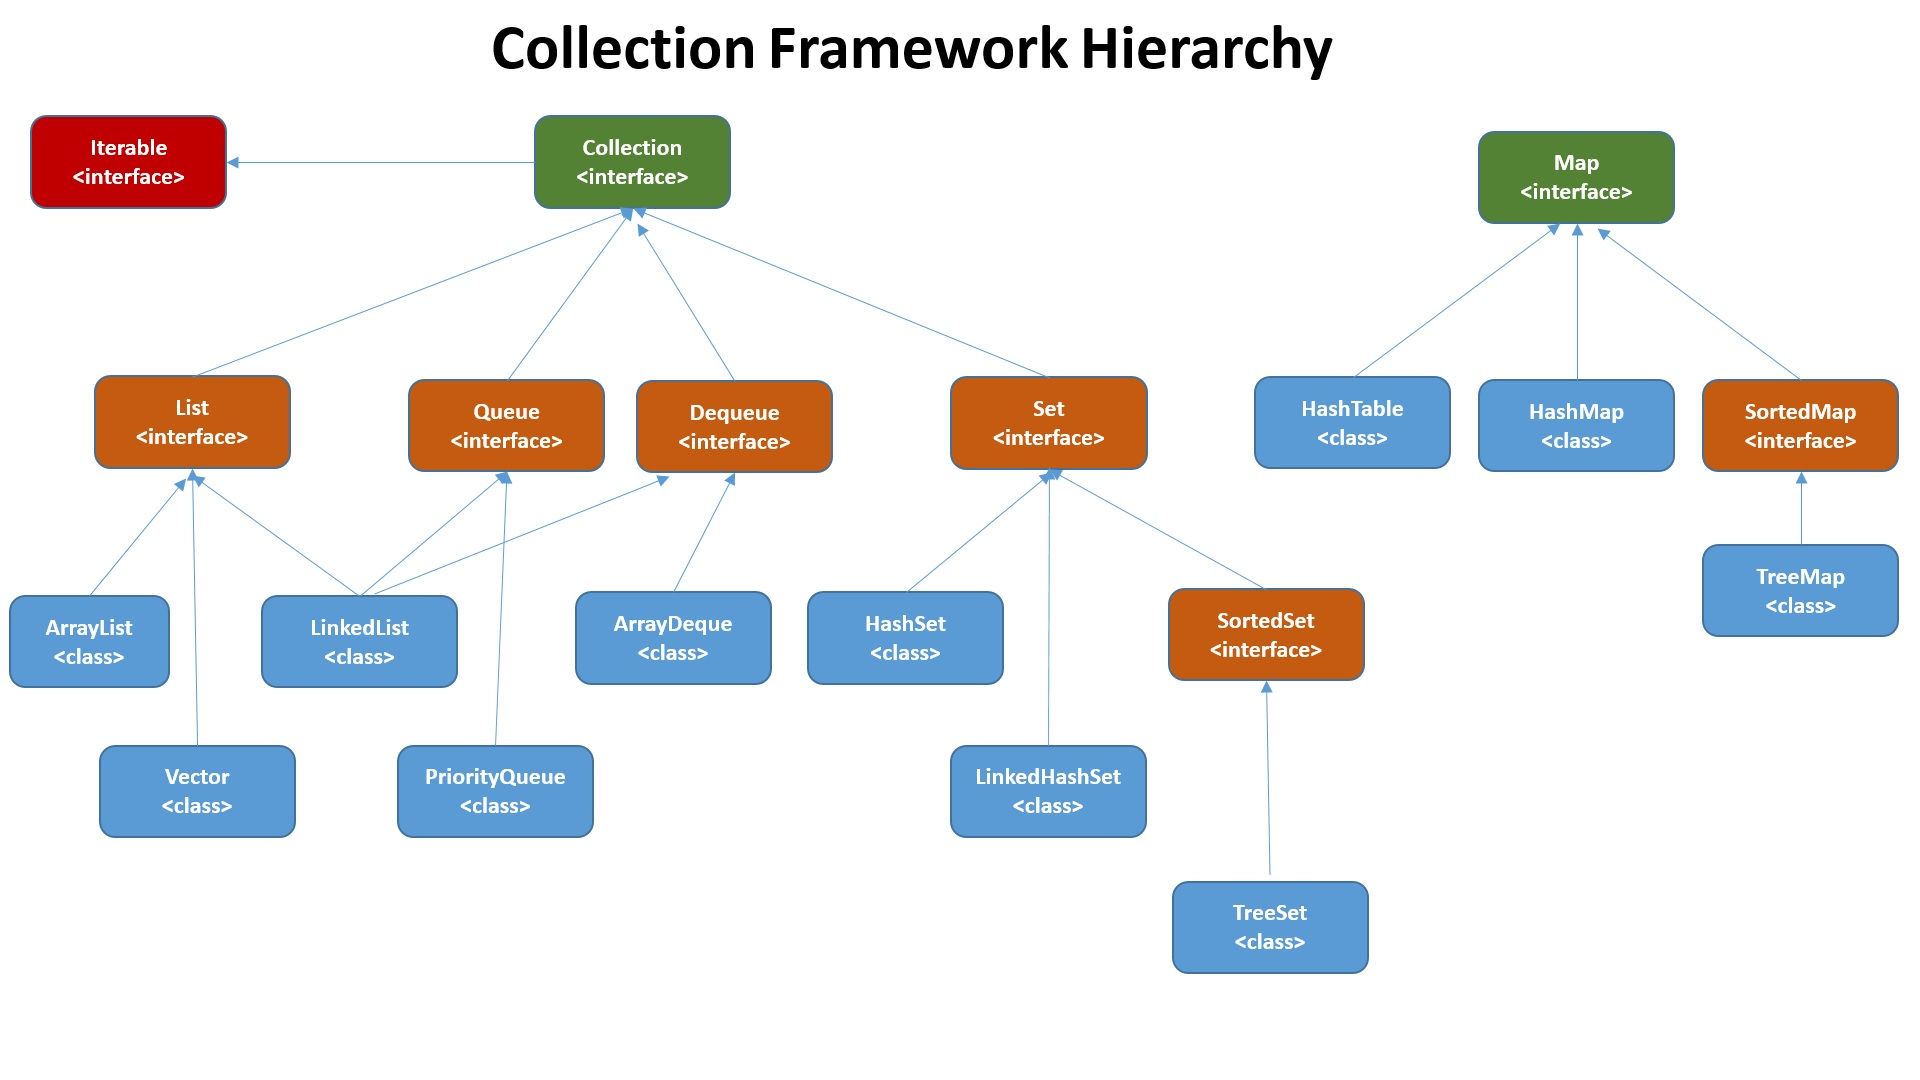
\includegraphics[width=\linewidth]{img/java-collection.jpg}
  }{
    Source: \url{https://facingissuesonit.com/2019/10/15/java-collection-framework-hierarchy/}
  }
\end{figure}

Also, \texttt{hashCode()} and \texttt{equals()}, important methods for these collections to work properly, were discussed. It was shown what they are and why we use them.

\subsubsection{OOP}

This part covered the basics and principles of Object Oriented Programming (OOP).

We started by discussing the basics, such as scopes, constructors, access modifiers, setter and getter methods, method overloading, and static methods. Since I was familiar with concepts from the CENG 242: Programming Language Concepts, I did not have a hard time with these concepts.

After the basics, we moved into the principles. We started with inheritance and class hierarchy. Here, I learned what superclasses and subclasses are and that Java does not support multiple inheritances. Furthermore, behaviors of some concepts, such as access modifiers and constructors, in inheritance are discussed. Also, other principles of abstraction, encapsulation, and polymorphism are covered, but I did not learn new information.

\subsubsection{JavaBeans and JDBC}

The last day of the week, when we got out of the basics of Java and learned databases and database connections by using Java, was a day that I learned new information and was challenged for the first time this week.

We started by talking the JavaBeans, which is a standard. By learning and reading about JavaBeans, I realized that many things are standardized in Java, and implementations are competed instead of the standards. This makes the reason why Java is exceptionally preferred in corporate areas clear.

Since we would have needed to add some dependencies and Maven would be used in our projects, we talked about Maven, a build automation tool, and installed it in addition to MySQL, which was going to be used as a database. After the installations and the environment adjustments, we dived into the Java Database Connectivity (JDBC), Java API that mainly manages connecting to a database. Connecting to a database, executing queries, using of ``\texttt{Statement}'', ``\texttt{ResultSet}'' and ``\texttt{PreparedStatement}'' which are basically used to sending SQL statements to databases, and transaction management.


\subsection{Git \& Bitbucket}

To our use during the internship, we were provided a Bitbucket account. We were asked to use Git and ``\textit{push}'' our codes to Bitbucket. Since we were asked to use Git, the basics and primary usage of Git and Bitbucket were shown. 


% \noindent Additionally, the OOP examples are done:
% \begin{itemize}
%   \item \textbf{ExampleThePen:} Constructors, Set and Get methods, Shadowing, \texttt{static} keyword.
%   \item \textbf{ExampleBusReservation:} Constructors, Set and Get methods, Shadowing, \texttt{static} keyword, Enumerations.
% \end{itemize}

% Example of the topic: \texttt{ExampleException}, Example IO

% The example \texttt{ExampleOccurrencesOfWords} is done.

% Some days, Some friends was talking about design patterns. In the third day of my internship, two people talked about two different design patterns, which are \textit{Adepter} and \textit{MVC} design patterns.

% New projects are opened after Inner Class part: \texttt{JIP-JDBC}.

% After these concepts are disccussed, example named \texttt{ExamplePenRevisited} is done.

% We have done the example named \texttt{ExampleInterfacePen}.

% Second Week
\section{Introduction to Web Development}

The first week of my internship was about the \texttt{Java} Core, whereas we focused on the enterprise version of \texttt{Java}, \texttt{Java EE}, or \texttt{Jakarta EE}, and web development in the second week.

\subsection{Introduction to \texttt{Java EE} Platform}

After learning the \texttt{Java} versions and their primary concern, we discussed enterprise-level applications and their needs. Then, we focused on how \texttt{Java} values developers, vendors, and businesses. Our mentor mentioned that the specifications are determined and defined concurringly, and vendors only compete at their implementation level in the \texttt{Java} world so that developers can use any \texttt{J2EE} implementation for development and deployment.

Additionally, I learned about layers that are the foundation of software architecture (presentation, application/business, data, and service layers) and types of software architectures (one-tier, two-tier, three-tier, and N-tier architectures) and their advantages and disadvantages.

\subsection{Introduction to Web Development on \texttt{Java} Platform}

After learning what websites and web applications are and their differences, we discussed web servers and installed one of the preferred web servers on \texttt{Java} World: `\texttt{Tomcat}'. Then, we focused on the basics, such as HTTP and WWW, Request and Response, DNS, of the web world.

After these basics, we learned the `\texttt{Servlets}', the basic concept and tool for Web development on \texttt{Java} world and \texttt{JSP}, which enables mixing static HTML content with unique code that produces the dynamic content.

\subsection{Developing \texttt{Java} Web Applications}

We learned the basic anatomy of a web application and web module structure. I believe these topics are pretty beneficial because knowing the web module's structure is essential in portability's development and deployment process. After that, we dived into HTTP and I was mainly surprised when I learned the greatness of the contents carried by a request and response. Then, we focused on Servlets which are the main fragment of \texttt{Java} web development. 

Additionally, we discussed the `\textit{Threading Issues}' caused by the multi-threaded approach, which is an approach to solving the problem of how one servlet object serves many clients. In this approach, instead of creating multiple things, the servlet container creates a separate thread for each invocation of \texttt{service()} method, and that thread runs all servlet methods.

We also discussed information-sharing techniques among servlets (ServletContext object, HttpSession object, Request attributes). Before learning these techniques, I used incredible nonsensical methods such as different web pages to carry information. However, these techniques are beneficial and make it easier to carry information between servlets.

\subsection{More on \texttt{Java} Web Applications}

We learned what a developer should do for an exception and error management by configuring a web descriptor, namely \texttt{web.xml}. This week, we generally used XML files for configurations; however, following weeks, we used annotation-based configurations.

We focused on session management and filters on the week's last days. We learned session tracking techniques in detail, which of them are tracking via IP address, user authentication, hidden form fields, URL rewriting, and cookies. In the filters part, we learned how filters actually work with other parts of the server. Then, we practiced how requests are used for authentication and security purposes.

Until this week, my knowledge about web development was pretty limited, and I was a novice to the web at this point. Therefore, these topics were confusing but enthusiastic for me.

% Third Week
\section{\texttt{Spring} Framework}

After learning \texttt{Java} and the basics of web development, I was amused. In web development, our next step was a framework. In the internship program, \texttt{Spring}, \href{https://spring.io/why-spring}{the world's most popular \texttt{Java} framework}, is chosen for that purpose. \texttt{Spring} is an open-source framework developed for \texttt{Java}. Generally, it is used for developing web apps with the \texttt{Java} Enterprise platform.

\subsection{Environment Setup}

Firstly, we prepared the environment by installing Apache Tomcat -\texttt{Java} servlet container- and Maven -software project management and comprehension tool. 

Since we will have been using the Maven, our mentor talked about \texttt{Maven}. We discussed what Maven is and how we can use it. Then, we briefly introduced \texttt{Spring} by mentioning what it is and why we use it.

This week was mainly about the \texttt{Spring} framework. I learned a lot of information about \texttt{Spring} this week. For ease of reading, I will dive into the subsections and briefly explain what I learned this week and what they are.

\subsection{Introduction to \texttt{Spring}}

% Dividing into the Spring
By using \texttt{Spring initializr}, we created our first spring project. While creating a project, our mentor addressed the features of \texttt{Spring initilizr} and the dependencies part of it. After we opened the project, our mentor firstly focused on the dependencies and their management. While discussing the dependencies, we found a problem with versions; therefore, our mentor talked about the general versioning methods. When we ran the app for the first time, some team members encountered a problem with the port of the application; hence, our mentor needed to show us how we could change the settings of the projects by using the application.yaml file of the project, configuration file of the \texttt{Spring}.

\subsubsection{Controllers}

% Controllers 
We started with the controllers. Controllers are part of the Spring Web model-view-controller (MVC) framework and meet the requests. By using the mapping annotations, requests are mapped to related functions inside the controller class. The functions usually return a response after necessary processes are done according to the request. In our projects, we usually used ``ResponseEntity'' classes because we returned an entity.

\subsubsection{Filter and Interceptor}

% Filter and Interceptor
We continued with the filters. The filters are objects used to intercept the HTTP requests and responses of the application. Basically, they are the layer before sending the request to the controller and before sending a response to the client. Some common usages are logging requests and responses, logging request processing time, formatting request body or header, verifying authentication tokens, or compressing responses.

Interceptors are pretty similar to filters, but they act in \texttt{Spring Context}, so they are powerful enough to manage HTTP Request and Response but can implement more sophisticated behavior because they can access all \texttt{Spring} contexts. In other words, we can not use filters outside the web context, while \texttt{Spring} interceptors can be used anywhere because they are defined in the application context.

\subsubsection{Exception}

% Exception
Then we dived into the exceptions. Firstly, we examined the default answer of \texttt{Spring} for errors. An example from my final project is given below. 
\begin{minted}[breaklines]{json}
{
  "timestamp": "2022-09-17T10:03:08.250+00:00",
  "status": 500,
  "error": "Internal Server Error",
  "trace": "tr.com.obss.jip.springfinal.exception.UserNotFoundException: User, whose id number is 99, is not found! ...",
  "message": "User, whose id number is 99, is not found!",
  "path": "/users/99"
}
\end{minted}

It can be said that this type of answer constitutes a security vulnerability because of the information the error provides an error message and codes. For example, someone can tell that this system uses the \texttt{Spring} framework. After examining the default answer of \texttt{Spring}, we realized errors are also needed to be handled due to security as well as providing a meaningful message. We discussed how we could handle errors and change the behaviors and messages when an error occurs.

\subsubsection{Model, Entity, and Database}

% Model
After the error handling, we learned the Data Transfer Objects (DTOs), which are used to encapsulate data and carry this data between processes and their usages. I extensively used models in the final project to transfer data between processes and layers.

% Entity and Database
Since we will have been using the database, we had to make the database connection. \texttt{Spring} provides database connection capability with hibernate, which is integrated inside \texttt{Spring} and makes the database connection and necessary database operation. 

Hibernate can also create the tables in the database by using entities provided by entity classes. Therefore, we used entity classes to tell the hibernate to create the table in the database.

\subsubsection{Services, Repositories, and Configuration}

% Services and Repositories
Services are generally used for business logic, such as creating, storing, or changing data. I extensively used the services in my final project. After the controller met the request, the proper function was called, and the necessary business was done in the project.

Repositories are the mechanism for encapsulating storage, retrieval, and search behavior that emulates a collection of objects. They are used for the access layer for accessing and making necessary operations in the database. We chose to use \texttt{Spring Data JPA} for this purpose. After making the required settings from the application.yaml, \texttt{Spring} automatically connects itself to the database and gets ready to execute queries with little effort. In repositories, there is almost no need to write SQL queries executed in the database, even if it is allowed. By using the specific combination of some keys in the function names inside the repository interface, we provide necessary information to \texttt{Spring} so that \texttt{Spring} can create the proper queries and execute them by connecting to the database.

% Various Configuration
After the basics, we dived into the configuration of our apps, such as security, password encryption, or data loading when it is started.


% Fourth Week
\section{\texttt{React}}

On the last day of the third week, we started discussing \texttt{React}, a user interface library created by Facebook on \texttt{JavaScript}. I had almost no experience with both \texttt{React} and \texttt{JavaScript}. 

\subsection{MPA and SPA}

% MPA and SPA
We started the discussion with MPA (multiple page applications) and SPA (single page applications) and why SPA should be chosen over MPA. \texttt{React} helps developers to develop SPA by using JavaScript and virtual DOM. Since our primary concern will have been learning \texttt{React}, we talked about its advantages and limitations and compared \texttt{React} with other frameworks and libraries by looking at the trends to have a better perspective.

% Rendering UI
We started with the \texttt{React} elements and continued with how we could render them. After learning the basics, we talked about JSX, a syntax extension to JavaScript that allows \texttt{React} elements to be written inside JavaScript using HTML tags. Since JSX has many different features, such as styling the elements and inserting JavaScript variables, we had to spend much time on it solving mini coding challenges.

\subsection{Functional and Class Components}

% Functional components and class components
\begin{wrapfigure}{r}{0.3\textwidth}
  \centering
  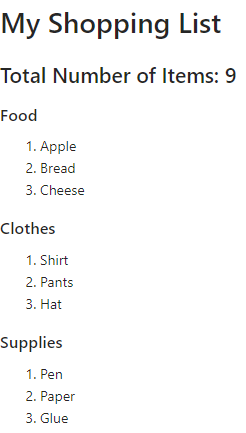
\includegraphics[width=0.3\textwidth]{img/shopping-app.png}
  \caption{Basic Shopping List App}
\end{wrapfigure}
We moved into components. A \texttt{React} component can be defined as an independent, reusable component that outputs the \texttt{React} element. We compared the class and functional components and discussed their usage differences. I realized that I tended to use class components because of the OOP and class familiarities, although functional components are excessively used in the sector.

After these, we solved an example, which can be called Shopping List App. It was a simple shopping list without adding or removing options, but it only showed the provided list. After we coded the exercise, our mentor also coded the exercise to show us another perspective.

\subsection{States}

% States
Then we discussed a crucial topic and feature of \texttt{React}: \texttt{States}. We talked about what a state is and how it is used. We then jumped into another critical issue in states: setting/updating the state. We realized and learned how to fix the different behaviors of setting states.

\subsection{Life Cycle Methods}

% Life Cycle Methods
Another essential topic was the life cycle methods of class components. While rendering and mounting the component, \texttt{React} runs various methods on the components at multiple phases. Life cycle methods can be used for specific purposes according to phases.

\subsection{Event Handlers}

% Event Handlers
Event handling is pretty similar to HTML events. We discussed that we could achieve some effects by using event handlers. For example, sending a request when a button is clicked or changing the state of a variable when a key is pressed can be achieved by event handlers.

\subsection{Promises, Back-end Requests, and JWT}

% Promises and Back-end Request
After the basics and some advanced topics, we moved into the back-end requests. Before talking about them, we discussed the promises, a feature of JavaScript. For back-end requests, we conversed about Axios. Axios provides support to different request types and configs and is easy to use.

% JWT
We briefly discussed JWT tokens used for token-based authentication instead of password authentication every time.


\end{document}